\scanpage{94}
\deleted{Écrivons les antipodiques des $s_i,s_3',s_3''$}
\[
\left\{\begin{aligned}
&\deleted{\underline a s_0=(1,-\frac1\alpha,-\frac1\alpha)=(1,-1-\alpha,-1-\alpha)=(1,\unsure{\alpha'},\alpha')}\\
&\deleted{\underline a s_1=(0,-\frac1\alpha,-\frac1\alpha)=(0,-1-\alpha,-1-\alpha)=(0,\alpha',\alpha')}\\
&\deleted{\underline a s_2=(1,-\frac1\alpha-1,-\frac1\alpha)=(1,-2-\alpha,-1-\alpha)=(\unsure{1|\alpha'},\alpha'-1,\alpha')}\\
&\deleted{\underline a s_3=(1,-\frac1\alpha,-\frac1\alpha-1)=(1,-1-\alpha,-2-\alpha)=(1,\alpha',\alpha'-1)}\\
&\deleted{\underline a s_3'=(2+\alpha,-2(1+\alpha),-(2+\alpha))=(1-\alpha',-2\alpha',\alpha'-1)}\\
&\deleted{\underline a s_3''=(1,-2(1+\alpha),-(2+\alpha))=(1,2\alpha',\alpha'-1)}
\end{aligned}\right.
\tag*{\deleted{(18)}}
\]
% Horizontal separator below the cancelled calculation, arrow at its left end.
\figure{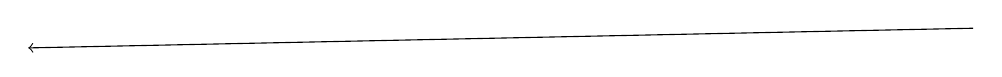
\begin{tikzpicture}\draw[<-] (0,0)--(12,.25);\end{tikzpicture}}

On aimerait prouver que \inserted{(sur un corps de base \unsure{quelc.})} trois \deleted{pts} \inserted{sommets} distincts \inserted{(\unsure{ce qui implique|non antipodiques} \unsure{provenant d'une arête|incidents à une arête} \unsure{par un pt donné})} ne sont pas alignés, et quatre points distincts ne sont pas \deleted{sur} \inserted{ds} un $=$ plan \uline{sauf} s'ils \deleted{appartiennent à une face} sont incidents \inserted{combinatoirement} à un $=$ sommet (ce qui implique qu'un sommet n'est incident \inserted{géom\textsuperscript{t}} à une face que s'il \deleted{elle} l'est combinatoirement; et \inserted{par suite} qu'une arête n'est incidente \inserted{géom\textsuperscript{t}} à une face que si elle est incidente combinatoirement).
\margin{?}
\margin{C'est en tous cas \uline{faux} en car. 2 !}
\figure{\begin{tikzpicture}\fill (0,.5) circle (1.5pt);\draw[->] (.15,.5)--(1.4,.55);\fill (0,0) circle (1.5pt);\draw (0.15,0)--(1.4,.1);\draw[->] (.7,1.4)--(2,2.6);\draw (1.95,2.75)--(1.75,5.2);\end{tikzpicture}}

Pour le premier pas, il y a trois vérifications à faire

\unsure{a)} La droite qui joint $s_0$ à son antipodique $\underline a s_0$ ne contient aucun autre sommet. i.e. \unsure{aucun des|aucun que les} \inserted{10} vecteurs \deleted{\unsure{tq}} \inserted{$(x,y,z)$} associés aux dix sommets distincts de $\unsure{s_3|s_0},\underline a s_0$, sont non prop. \unsure{au Centre|au vecteur}
\[
\underline a s_0=(\alpha',1-\alpha',1-\alpha')\deleted{\unsure{=(1,-1-\alpha,-1-\alpha)}}
\]
ou encore à
\[
\frac1{\unsure{\alpha'}}\underline a s_0=(1,\alpha',\alpha')
\]
% archive sheet number: 93
